\chapter{System Design}
\label{ch:design}

\section{Design Goals}
\label{sec:goals}

\begin{enumerate}[label=G\arabic*.]
  \item \textbf{Correct by construction, verified on data.} Designs are 3NF and lossless by the
  algorithm, and every apply re-checks losslessness on the real rows before committing.
  \item \textbf{SQL in plain sight.} No ORM: constraints, PL/pgSQL, triggers, views, dynamic SQL and
  catalog queries are hand-written, and the generated SQL is shown to the user.
  \item \textbf{Work where the data is.} Profiling, dependency checks and duplicate search run inside
  PostgreSQL; only the set algebra of synthesis runs in Python.
  \item \textbf{Isolation by privilege.} A user's query can reach only its own workspace because the
  database role lacks the privileges, not because the application filters text.
  \item \textbf{Non-destructive and auditable.} The raw import is never modified; every repair is a
  logged, transactional edit of a separate staging copy.
\end{enumerate}

\section{System Architecture}
\label{sec:architecture}

\InputIfFileExists{figures/architecture}{}{}

QLens is a three-tier web application whose bottom tier does unusually much work
(\cref{fig:architecture}). The \emph{client} is a React single-page application \cite{react}; it holds no
authoritative state and talks JSON to \code{/api/*} with the session in an \code{httpOnly} cookie. The
\emph{application tier} is FastAPI on Python 3.13 \cite{fastapi} with psycopg~3 \cite{psycopg}; each request
runs in one transaction on a pooled connection as the owning role \code{qlens\_app}, committed before the
response is sent so that a commit failure can never follow a success reply. The \emph{data tier} is a
private PostgreSQL 18 cluster \cite{postgres18docs} with the \code{qlens} metadata schema and, per
workspace, three schemas and one role:

\begin{itemize}
  \item \code{ws\_<id>\_src}: \code{\_raw} (every cell as text, never edited) and \code{\_staging}
  (typed, the only table clean-up edits);
  \item \code{ws\_<id>}: the generated 3NF tables and the \code{original\_sheet} view;
  \item \code{ws\_<id>\_lab}: a scratch copy for performance experiments (\stplan);
  \item \code{qlens\_ws\_<id>}: a \code{LOGIN}, \code{NOINHERIT} role with \code{CONNECTION LIMIT 3}, role-level
  settings that make every session read-only, stop statements after 5\,s and end idle transactions
  after 10\,s, and \code{USAGE}/\code{SELECT} on its own schemas
  only (with \code{ALTER DEFAULT PRIVILEGES} for future tables). Its password is an HMAC of the workspace
  id under the server secret, so it is never stored. Role and schemas are created in the same
  transaction as the workspace row and dropped with it.
\end{itemize}

\begin{table}[htbp]
\centering
\caption[Technology stack]{Technology stack.}
\label{tab:stack}
\small
\begin{tabularx}{\textwidth}{@{}l X@{}}
\toprule
Layer & Technology \\
\midrule
Database & PostgreSQL 18 (private cluster), PL/pgSQL, \code{pg\_trgm} \cite{pgtrgm} \\
Backend & Python 3.13, FastAPI, psycopg 3 with connection pool, pglast \cite{pglast}, openpyxl, argon2-cffi \\
Frontend & React 19, TypeScript, Vite, Tailwind CSS, TanStack Query, React Flow, CodeMirror \\
Testing & pytest against a real PostgreSQL test database; Vitest \\
\bottomrule
\end{tabularx}
\end{table}

\section{Detailed Design Methodologies}
\label{sec:detailed}

\subsection{Metadata Schema}
\label{sec:design-metadata}

QLens's own data is a normalized design of 22 tables plus a migrations log (\cref{fig:er}). Users own
workspaces; a workspace holds at most one dataset (\code{UNIQUE workspace\_id}); a dataset has columns,
candidate keys, functional dependencies, duplicate groups and a log of fixes; designs are
\tbl{schema\_proposals} with their \tbl{proposed\_tables}, \tbl{proposed\_columns} and unique keys; and
the query side records saved queries, runs, plans and index experiments. Multi-column keys and
dependency left-hand sides are junction tables (\tbl{candidate\_key\_columns}, \tbl{fd\_lhs\_columns}),
so no column stores a list of column names. The only redundancy is deliberate and documented: for
example \code{dataset\_id} is kept next to \code{column\_id} for cheap filtering and cascades.

\InputIfFileExists{figures/er}{}{}

\begin{table}[htbp]
\centering
\caption[Integrity rules]{Selected integrity rules enforced by the metadata schema.}
\label{tab:integrity}
\small
\begin{tabularx}{\textwidth}{@{}>{\raggedright\arraybackslash}p{0.56\textwidth} X@{}}
\toprule
Rule & Purpose \\
\midrule
\code{CHECK (status <> 'applied' OR lossless\_ok IS TRUE)} & a design cannot be recorded as applied without a passed check (\code{IS TRUE}: NULL must fail) \\
partial \code{UNIQUE (dataset\_id) WHERE status = 'draft'} and \code{\dots{} = 'applied'} & at most one draft and one applied design per dataset \\
\code{is\_exact}, \code{violation\_ratio}, \code{speedup} \code{GENERATED \dots{} STORED} & derived values can never disagree with their inputs \\
\code{CHECK ((role = 'fk') = (references\_table\_id IS NOT NULL))} & a column is a foreign key exactly when it references a table \\
\code{CHECK (name \textasciitilde{} '\textasciicircum[a-z\_][a-z0-9\_]\{0,62\}\$')} & every stored name is a safe identifier within 63 bytes \\
\code{ON DELETE CASCADE} / \code{SET NULL} & no orphans; run history survives deleting a saved query \\
index \code{query\_runs (workspace\_id, created\_at DESC)} & serves the history page and the summary view (foreign keys are not indexed automatically, so each FK has a covering index) \\
\bottomrule
\end{tabularx}
\end{table}

\paragraph{Triggers and views.} \code{touch\_updated\_at} stamps \code{updated\_at} with
\code{clock\_timestamp()} on every update. \code{record\_query\_run} (\cref{lst:trigger}) keeps a saved
query's counters in step with its successful runs; its \code{WHEN} clause filters before the function is
called. \code{v\_workspace\_summary} feeds the dashboard through two \code{LEFT JOIN LATERAL} aggregates,
\code{v\_slow\_queries} uses \code{percentile\_cont(0.9) WITHIN GROUP}, and \code{v\_saved\_query\_trend}
uses the window functions \code{row\_number}, \code{lag} and a five-run moving \code{avg}.

\begin{lstlisting}[caption={[Run-recording trigger]AFTER INSERT trigger maintaining saved-query statistics (\code{002\_logic.sql})},label={lst:trigger}]
CREATE FUNCTION qlens.record_query_run() RETURNS trigger LANGUAGE plpgsql AS $$
BEGIN
    UPDATE qlens.saved_queries
       SET run_count = run_count + 1, last_run_at = NEW.created_at,
           last_duration_ms = NEW.duration_ms
     WHERE id = NEW.saved_query_id;
    RETURN NULL;
END $$;
CREATE TRIGGER query_runs_record AFTER INSERT ON qlens.query_runs
    FOR EACH ROW WHEN (NEW.saved_query_id IS NOT NULL AND NEW.status = 'ok')
    EXECUTE FUNCTION qlens.record_query_run();
\end{lstlisting}

\subsection{Dependency Discovery}
\label{sec:design-discovery}

\InputIfFileExists{figures/pipeline}{}{}

\Cref{fig:pipeline} shows the pipeline. Import copies every cell into \code{\_raw} with \code{COPY},
infers each column's type with one aggregate query of regular-expression tests (dates through the
PL/pgSQL function \code{try\_date}, which returns NULL instead of raising), and builds \code{\_staging}
with \code{CREATE TABLE \dots{} AS SELECT} and the casts.

Discovery then asks PostgreSQL. \code{qlens.check\_fd} (\cref{lst:checkfd}) groups the staged rows by
the left-hand side and the right-hand side and returns, for $X \rightarrow A$, the number of rows that
would have to change for the dependency to hold: per $X$-group, every row except those with the most
frequent $A$. This is the $g_3$ error measure of approximate dependencies \cite{kivinen1995}. A
dependency is \emph{exact} at 0 and \emph{approximate} up to 2\% of the rows, and it must be supported by
at least two repeated $X$-groups. Identifiers enter only through \code{format('\%I')}, so the dynamic SQL
cannot be injected. Candidate keys use \code{qlens.is\_unique} on combinations of 1--3 columns, pruned
first by the profile: a key must have no NULLs, and the product of its columns' distinct counts must
reach the row count.

\begin{lstlisting}[caption={[Dependency check in PL/pgSQL]\code{qlens.check\_fd}: measuring a dependency with dynamic SQL (\code{004\_analysis.sql})},label={lst:checkfd}]
CREATE FUNCTION qlens.check_fd(p_schema text, p_table text, p_lhs text[], p_rhs text)
RETURNS TABLE (row_count bigint, lhs_values bigint, repeated_groups bigint, violating_rows bigint)
LANGUAGE plpgsql STABLE AS $$
DECLARE
    t   text := format('%I.%I', p_schema, p_table);
    lhs text;
BEGIN
    SELECT string_agg(format('%I', c), ', ') INTO lhs FROM unnest(p_lhs) AS c;
    RETURN QUERY EXECUTE format(
        'WITH c AS (SELECT %1$s, %2$I, count(*) AS cnt FROM %3$s GROUP BY %1$s, %2$I), '
        '     g AS (SELECT %1$s, sum(cnt) AS n, max(cnt) AS keep FROM c GROUP BY %1$s) '
        'SELECT (SELECT count(*) FROM %3$s), count(*), count(*) FILTER (WHERE n >= 2), '
        '       coalesce(sum(n - keep), 0)::bigint FROM g',
        lhs, p_rhs, t);
END;
$$;
\end{lstlisting}

Raw discovery is noisy, so three rules keep the list readable: measures (amounts, quantities) and flags
are never determinants; a pair $XY \rightarrow A$ is dropped when $X$ alone already (nearly) determines
$A$; and an approximate $X \rightarrow A$ explained by an exact $X \rightarrow Z$ and $Z \rightarrow A$
is reported only once, at its root. Dependencies implied by the others are flagged \emph{derived}. On
the fee register this leaves exactly six core dependencies, two of them approximate: 8 rows for
\fd{student\_phone}{student\_name} and 5 for \fd{teacher}{teacher\_phone}.

\subsection{Data Cleaning}
\label{sec:design-cleanup}

\paragraph{Near-duplicates.} Spellings equal after lower-casing and collapsing spaces and full stops are
certain duplicates. Probable typos are found with \code{pg\_trgm} trigram similarity \cite{angell1983}:
candidate values go into a temporary table with a GIN \code{gin\_trgm\_ops} index, so the \code{\%}
operator finds look-alikes without comparing every pair. Two rules remove false alarms: values whose
digits differ are different things (\emph{Foundation 9} and \emph{Foundation 10}), and a typo must be at
most a third as frequent as the spelling it resembles. Matches are clustered with union--find.

\paragraph{Inconsistencies and repairs.} Each approximate dependency lists its conflicting groups with the
most frequent value as the suggestion, which is the minimal repair under $g_3$. A merge or fix is one
\code{UPDATE} of \code{\_staging} inside a transaction (\code{FOR UPDATE} on the affected rows), logged in
\tbl{dataset\_fixes} and followed by re-profiling; ``accept all'' merges every certain duplicate, fixes
every approximate dependency and re-analyzes, so both fee-register inconsistencies become exact.

\subsection{3NF Synthesis}
\label{sec:design-3nf}

The design is built from exactly the dependencies the user sees: exact, accepted and not derived.
Synthesis is set algebra over column names, implemented in Python and summarized in
\cref{alg:bernstein}. The closure $X^{+}$ answers every question it needs: $X \rightarrow A$ follows from
$F$ iff $A \in X^{+}$ \cite{armstrong1974}. The minimal cover splits right-hand sides, removes extraneous
left-hand attributes and redundant dependencies, with all tie-breaks in sheet order so the result is
deterministic. Groups with equivalent determinants are merged, and Bernstein's step 5 then prunes
dependencies made redundant by the equivalences \cite{bernstein1976}.

\InputIfFileExists{figures/bernstein}{}{}

Plain synthesis preserves dependencies but is lossless only if some relation contains a key of the
whole table \cite{biskup1979}. QLens therefore designates as \emph{fact} relation the relation that
contains every undetermined attribute and whose closure is the whole table, or else adds one built from a
key of the dependencies. Joining outward from the fact relation, each join is on a key of the relation
being joined, so it adds determined attributes and never adds or removes rows. 900 randomized cases are
checked against a chase-based lossless-join test \cite{aho1979} and a brute-force 3NF test.
\Cref{fig:fee-example} shows the result for the fee register.

\InputIfFileExists{figures/fee-example}{}{}

\subsection{Proposal and Apply}
\label{sec:design-apply}

\paragraph{From relations to tables.} \stdone{} Every table gets
\code{id bigint GENERATED ALWAYS AS IDENTITY PRIMARY KEY}; its determinant and equivalent determinants
become \code{UNIQUE NULLS NOT DISTINCT} constraints, so an empty \emph{Teacher} cell is one teacher stored
once. When a relation contains another entity's natural key, those columns are replaced by a foreign key
\code{<entity>\_id ... ON DELETE RESTRICT}, \code{NOT NULL} exactly when the replaced columns had no empty
cells. Tables are named from their determinant (\code{student\_name} $\rightarrow$ \tbl{students}), carry a
plain-English explanation and can be renamed while the proposal is a draft (otherwise 409
\code{proposal\_not\_draft}). The SQL is generated in topological order of the foreign keys: entity loads
are \code{INSERT \dots{} SELECT DISTINCT} from \code{\_staging}, foreign keys are looked up by natural key
(plain \code{=} where the key has no NULLs, so a hash join is possible, \code{IS NOT DISTINCT FROM}
otherwise), the fact keeps every row in sheet order, and the view \code{original\_sheet} joins everything
back into the original columns.

\paragraph{One transaction.} \stdone{} Apply locks the draft with \code{SELECT \dots{} FOR UPDATE}, drops
and recreates the workspace schema, runs the generated statements and finally the check of
\cref{lst:lossless}. A non-zero count raises 409 \code{lossless\_check\_failed} with up to five differing
rows, and PostgreSQL rolls everything back: old tables and statuses are untouched. Otherwise the previous
applied proposal is set to \emph{superseded} \emph{before} the new one becomes \emph{applied}, since the
partial unique indexes allow only one applied design per dataset, and after the commit each new table is
\code{ANALYZE}d so that the first queries get real statistics.

\begin{lstlisting}[caption={[Lossless check]The lossless check generated for the fee register (column list abbreviated as \code{cols})},label={lst:lossless}]
SELECT (SELECT count(*) FROM ws_20_src._staging)  AS staging_rows,
       (SELECT count(*) FROM ws_20.original_sheet) AS reconstructed_rows,
       (SELECT count(*) FROM (SELECT cols FROM ws_20.original_sheet
                              EXCEPT ALL SELECT cols FROM ws_20_src._staging) d) AS extra_rows,
       (SELECT count(*) FROM (SELECT cols FROM ws_20_src._staging
                              EXCEPT ALL SELECT cols FROM ws_20.original_sheet) d) AS missing_rows;
\end{lstlisting}

The comparison is of \emph{multisets}: \code{EXCEPT} would hide a duplicated or lost copy of a repeated
row, while \code{EXCEPT ALL} cancels rows one for one; and both directions are needed, because
$A$ \code{EXCEPT ALL} $B$ is empty whenever $A \subseteq B$. On the cleaned fee register all 3{,}000 rows
come back exactly, with 6 teachers, 8 batches and 300 students. Tests also cover forced failures,
reserved-word headers (\emph{Order}, \emph{Group}, \emph{User's Name}), empty determinants, the other two
samples and randomly generated sheets (a 400-seed run passed throughout).

\subsection{Query Sandbox}
\label{sec:design-sandbox}

\InputIfFileExists{figures/sequence-query}{}{}

\stwip{} A user query never runs on the application's pooled connection (\cref{fig:seq-query}). After the
workspace is checked to belong to the session's user and the text is parsed with pglast (one
\code{SELECT}, no forbidden functions), it runs on a separate login as \code{qlens\_ws\_<id>} in a
read-only transaction with a statement timeout, and at most 1{,}000 rows are returned. The outcome is then
recorded in \tbl{query\_runs} on the pooled connection, where the trigger of \cref{lst:trigger} updates the
saved query. The role, its settings, its grants, \tbl{query\_runs} and the trigger are built and tested;
the runner and its editor are being completed.

\subsection{Interface and Assistant}
\label{sec:design-ui}

Each generated table keeps one lane colour (\code{proposed\_tables.color\_index}) across the Analyze
diagram, the ER canvas, the SQL and these figures. The landing page, dashboard and Analyze screen are
\stdone: Analyze opens with a diagram of the sheet's structure, a banner of candidate keys and a graph of
dependencies, solid when exact and dashed when approximate (\cref{fig:analyze}). Motion explains rather
than decorates: diagrams enter in stages, only \code{transform}, \code{opacity} and
\code{stroke-dashoffset} are animated, and everything is static under \code{prefers-reduced-motion}.

\begin{figure}[htbp]
  \centering
  \IfFileExists{screenshots/analyze-issues-dark.png}{%
    \fcolorbox{rule}{white}{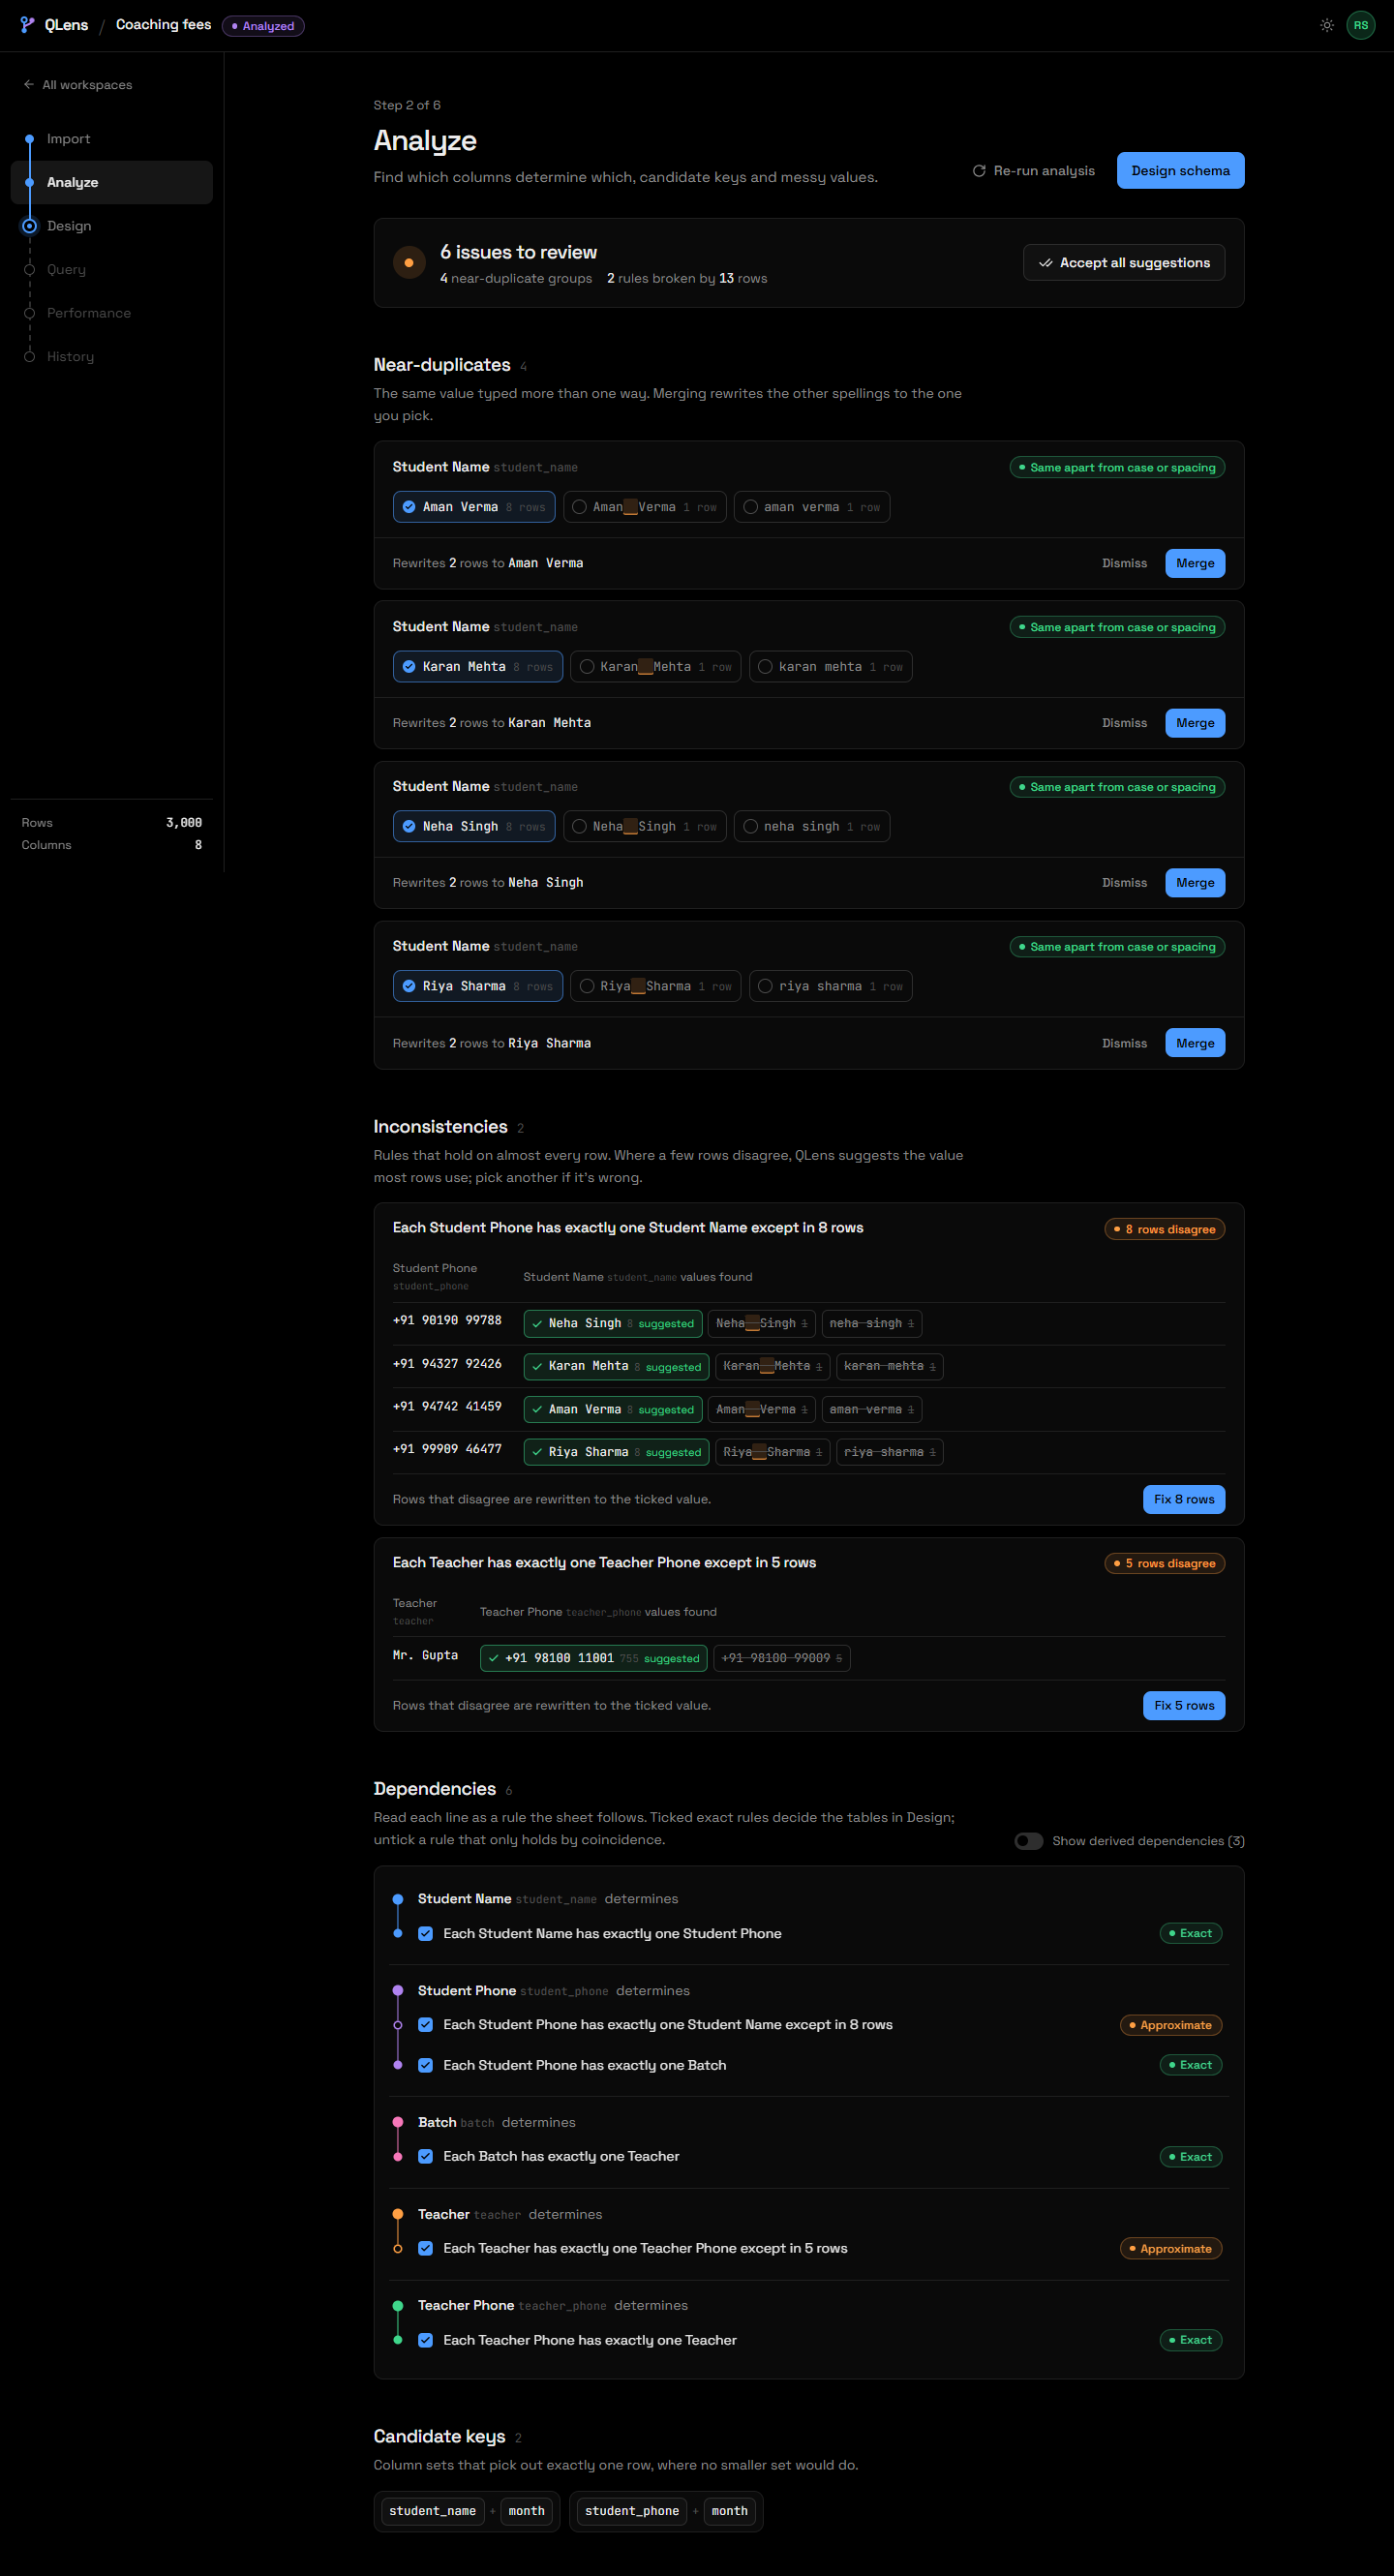
\includegraphics[width=0.68\linewidth]{screenshots/analyze-issues-dark.png}}}{}
  \caption[Analyze screen]{Analyze: candidate keys, the dependency graph (dashed edges are approximate) and
  the issues with their suggested fixes.}
  \label{fig:analyze}
\end{figure}

\stwip{} The Design step is a dot-grid canvas with draggable, lane-coloured tables, inline renaming, a
``why this design'' panel, the SQL and the Apply button; its backend is complete. On it floats the
command bar of the optional Gemini assistant. The model chooses, by function calling, between answering a
question and reworking the draft, but it can act only through server-validated tools:
\code{describe\_schema}, \code{check\_dependency} (which runs \code{qlens.check\_fd}), \code{run\_sql}
(through the sandbox), \code{explain\_query}, \code{rename\_table}/\code{rename\_column} (same checks as
the user's renames), \code{set\_dependency\_accepted} (re-synthesizes) and \code{move\_column}, allowed only
when \code{check\_fd} shows the target's determinant determines the column exactly. Every edit creates a
new draft version, so it can be undone, and conversations and tool calls are stored in the \code{qlens}
schema.
